\newcommand{\teta}{\tilde{\eta}}

Incompressible flow represents the zero-Mach number limit of fluid
flow---no compressibility effects are modeled.  We can extend the
ideas of incompressibe flow to allow us to model some compressibility
effects, giving rise to low Mach number methods.

\section{Low Mach divergence constraints}

The key idea in solvers for low Mach number flows is that, as a fluid
element advects, its pressure remains the same as the background
state.  For an atmosphere, this background state is a hydrostatic
profile.  For a smallscale combustion flow, this background state is a
spatially constant pressure (and constaint-in-time if the domain is
open).  We'll denote this background pressure as $p_0(r,t)$, where 
$r$ is a radial coordinate.

We can derive the constraint on the velocity field by considering the
Lagrangian derivative of the pressure---this captures the change in
pressure of a fluid element as it moves through the domain.
\begin{equation}
\frac{Dp_0}{Dt} = \left . \frac{\partial p_0}{\partial \rho} \right |_s
     \frac{D\rho}{Dt} +
     \left . \frac{\partial p_0}{\partial s} \right |_\rho
     \frac{Ds}{Dt}
\end{equation}
we recognize that $\Gamma_1 \equiv \partial \log p_0/\partial \log \rho |_s$.
The Maxwell relations tell us that
\begin{equation}
\partial p_0/\partial s |_\rho = \rho^2 \partial T/\partial \rho |_s
\end{equation}
and $\partial T/\partial \rho |_s$ can be derived from the first law
of thermodynamics, giving:
\begin{equation}
\left . \frac{\partial p_0}{\partial s} \right |_\rho 
= \sigma \Gamma_1 p_0 T
\end{equation}
with 
\begin{equation}
\sigma = \frac{\partial p_0/\partial T |_\rho}{\rho c_p \partial p_0/\partial \rho |_T}
\end{equation}

From the first law of thermodynamics, we see
\begin{equation}
T \frac{Ds}{Dt} = \frac{De}{Dt} + p_0 \frac{D(1/\rho)}{Dt}
\end{equation}
which is our internal energy evolution equation.  The internal
energy in a fluid parcel can change due to local heat release and 
diffusion, so we can write:
\begin{equation}
T \frac{Ds}{Dt} = \frac{De}{Dt} + p_0 \frac{D(1/\rho)}{Dt} = H + \nabla \cdot (k \nabla T)
\end{equation}
where $H$ is the specific energy generation rate and $k$ is the 
thermal conductivity.  Putting this all together, we have:
\begin{equation}
\frac{Dp_0}{Dt} = \frac{\Gamma_1 p_0}{\rho} \frac{D\rho}{Dt}
   + \sigma \Gamma_1 p_0 \left [ H + \nabla \cdot k \nabla T \right ]
\end{equation}
The continuity equation gives us:
\begin{equation}
\frac{D\rho}{Dt} = -\rho \nabla \cdot U
\end{equation}
and we finally have:
\begin{equation}
\nabla \cdot U + \frac{1}{\Gamma_1 p_0}\frac{Dp_0}{Dt} = \sigma (H + \nabla \cdot k  \nabla T) \equiv S
\end{equation}
This is the general constraint equation for low Mach flow.  Note that the
only approximation we made is $p \rightarrow p_0$.

A useful limit is smallscale combustion.  In an open domain, we can take
$p_0$ as constant, so $Dp_0/Dt = 0$, and we are left with
\begin{equation}
\nabla \cdot U = S
\end{equation}
This looks like the constraint for incompressible flow, but with a source
to the divergence.  This source captures the compressible effects due
to local heat release---as a fluid parcel moves, the only changes to
its density will come through local heat release.

Another interesting case is that of an atmosphere.  If we consider an
ideal gas, then $\Gamma_1 = \gamma = \mathrm{constant}$.  A second
appromation we take is that $p_0 = p_0(r)$---i.e., no time
dependence to the atmosphere.  Finally, we'll consider the case
with no local heat sources ($S = 0$).  Then we have
\begin{equation}
\nabla \cdot U + \frac{1}{\gamma p_0} U \cdot \nabla p_0 = 0
\end{equation}
which is equivalent to
\begin{equation}
\nabla \cdot \left ( p_0^{1/\gamma} U \right ) = 0
\end{equation}
This constraint captures the changes in compressibilty due to the 
background stratification of an atmosphere.  If the structure of the
atmosphere is isentropic, then we know that $d\log p_0 = \gamma d\log \rho_0$,
where we use $\rho_0$ to represent the density corresponding to $p_0$, and
we can write this constraint as:
\begin{equation}
\nabla \cdot (\rho_0 U) = 0
\end{equation}
This is the traditional anelastic constraint.


\section{Asymptotics}



\section{Extending the incompressible algorithm}

The solution methodology for these low Mach number systems follows 
that of the incompressible flow, but with two additions.  First,
we need to incorporate a density (mass continuity) evolution equation.

Next, we need to be able to enforce more general forms of the 
divergence constraint, which as we'll see in a moment, require
us to solve a variable-coefficient elliptic equation.  Our
multigrid technique will need to be suitably modified.

\subsection{Density evolution}

We need to solve the continuity equation.  We use the same techniques
that were used for advection.  Our equation is:
\begin{equation}
\rho_t + (\rho u)_x + (\rho v)_y = 0
\end{equation}
The $x$-interface left state would be:
\begin{align}
\rho_{i+1/2,j,L}^{n+1/2} &= \rho_{i,j}^n + 
   \frac{\Delta x}{2} \frac{\partial \rho}{\partial x} +
   \frac{\Delta t}{2} \frac{\partial \rho}{\partial t} + \ldots \nonumber \\
%
 &= \rho_{i,j}^n + 
    \frac{\Delta x}{2} \frac{\partial \rho}{\partial x} +
    \frac{\Delta t}{2} \left [ -(\rho u)_x -(\rho v)_y \right ]_{i,j} \nonumber\\
%
 &= \rho_{i,j}^n + 
   \frac{\Delta x}{2} \left ( 1 - \frac{\Delta t}{\Delta x} u_{i,j} \right )
        \frac{\partial \rho}{\partial x}
   - \frac{\Delta t}{2} \rho u_x - \frac{\Delta t}{2} (\rho v)_y 
\end{align}
A similar construction would yield the right state at that interface. 
The Riemann problem is just upwinding:
\begin{equation}
\rho_{i+1/2,j}^{n+1/2} = \mathcal{R}(\rho_{i+1/2,j,L}^{n+1/2},
                                     \rho_{i+1/2,j,R}^{n+1/2}) =
  \left \{
  \begin{array}{cl}
     \rho_{i+1/2,j,L}^{n+1/2} & u_{i,j} > 0 \\
     \rho_{i+1/2,j,R}^{n+1/2} & u_{i,j} < 0 
  \end{array} \right .
\end{equation}
     



\subsection{Variable-coefficient elliptic equation}

\label{sec:lm:vcelliptic}

We now need to solve an elliptic equation of the form:
\begin{equation}
\nabla \cdot (\eta \nabla \phi) = f
\end{equation}

If we denote the discrete divergence and gradient operators as $D$ and $G$,
then our operator will be $L_\eta \equiv D \eta G$.  If we wish to
use a cell-centered discretization for $\phi$, then using a standard 
centered-difference for $D$ and $G$ will result in a stencil that reaches
two zones on either side of the current zone.  This can lead to an
odd-even decoupling. \MarginPar{cite the appropriate Bell paper}

\MarginPar{there is a Pao and Colella (or Pao's thesis?) that also 
discusses issues with cell-centered}

Instead, we again use an approximate projection.  We discretize the
variable-coefficient Laplacian as:
\begin{align}
(L_\eta \phi)_{i,j} = 
 & \frac{\eta_{i+1/2,j} (\phi_{i+1,j} - \phi_{i,j}) -
        \eta_{i-1/2,j} (\phi_{i,j} - \phi_{i-1,j})}{\Delta x^2} + \nonumber \\
 & \frac{\eta_{i,j+1/2} (\phi_{i,j+1} - \phi_{i,j}) -
        \eta_{i,j-1/2} (\phi_{i,j} - \phi_{i,j-1})}{\Delta y^2}
\label{lm:eq:lap}
\end{align}

We can define the interface values of $\eta$ as the averages of the
cell-centered values.  Our elliptic equation is then 
\begin{equation}
(L_\eta \phi)_{i,j} = f_{i,j}
\end{equation}

The relaxation method for this operator again relies on isolating
$\phi_{i,j}$, yielding:
\begin{equation}
\phi_{i,j} = \frac{\teta_{i+1/2,j}\phi_{i+1,j} + \teta_{i-1/2,j}\phi_{i-1,j} +
                   \teta_{i,j+1/2}\phi_{i,j+1} + \teta_{i,j-1/2}\phi_{i,j-1} -
                   f_{i,j} } 
                  {\teta_{i+1/2,j} + \teta_{i-1/2,j} + 
                   \teta_{i,j+1/2} + \teta_{i,j-1/2}}
\label{lm:eq:smooth}
\end{equation}
with the shorthand that $\teta_{i\pm1/2,j} = \teta_{i\pm1/2,j}/\Delta x^2$
and $\teta_{i,j\pm1/2} = \teta_{i,j\pm1/2}/\Delta y^2$.

To put this into our multigrid framework, there are three changes we
need to make:
\begin{itemize}
\item The smoothing function needs to implement the more general smoothing
described by Eq.~\ref{lm:eq:smooth}.

\item The residual function needs to compute $(L_\eta \phi)_{i,j}$ according
to Eq.~\ref{lm:eq:lap}, and then $r_{i,j} = f_{i,j} - (L_\eta \phi)_{i,j}$.

\item The coefficients, $\eta$ should be averaged to the edges on the fine
grid and then restricted down the multigrid hierarchy as edge-based 
quantities.
\end{itemize}

\subsection{Test problem}

\subsubsection{Periodic}

To test the solver, we need to devise a problem with a known analytic
solution.  The easiest way to do this is to pick an $\eta(x)$ and
$\phi$ and then do the divergence and gradients to find the required
righthand side, $f$.  We'll use periodic BCs, and for our
equation $\nabla \cdot ( \eta \nabla \phi ) = f$, the following
provide a well-posed test problem:
\begin{align}
\eta &= 2 + \cos(2\pi x) \cos(2\pi y)  \label{eq:vc:lap}
\\
f &= -16.0 \pi^2 \left [ \cos(2\pi x)\cos(2\pi y) + 1 \right ] \sin(2\pi x)\sin(2 \pi y) \nonumber
\end{align}
with the solution:
\begin{equation}
\phi^\mathrm{true} = \sin(2 \pi x) \sin(2\pi y) \nonumber \\
\end{equation}

There is an important caveat when dealing with a purely-periodic
problem.  Since there is no boundary values to ``anchor'' the solution,
it is free to float.  Solving the elliptic problem will give use the
correct $\nabla \phi$, but the average of $\phi$ over the domain is 
unconstrained.  For our algorithms, it is $\nabla \phi$ that matters
(that is the forcing term that enters into the momentum equation).

When for checking convergence, we want to compare to the exact solution.
We therefore normalize $\phi$ by subtracting off its average value before
computing the norm of the error with respect to the exact solution:
\begin{equation}
\epsilon = \| \phi_{i,j} - \bar{\phi} - \phi^\mathrm{true}_{i,j} \| \enskip ,
\end{equation}
where
\begin{equation}
\bar{\phi} = \frac{1}{N_x N_y} \sum_{i,j} \phi_{i,j}
\end{equation}
As discussed in \S~\ref{sec:multigrid:other}, this can arise if
the discrete form the righthand side, $f_{i,j}$ does not sum exactly
to zero.  Figure~\ref{fig:mg_vc} shows the solution to this problem
with a $512^2$ grid. and the convergence of the solver described
here is shown in Figure~\ref{fig:mg_vc_converge}.

\begin{figure}[t]
\centering
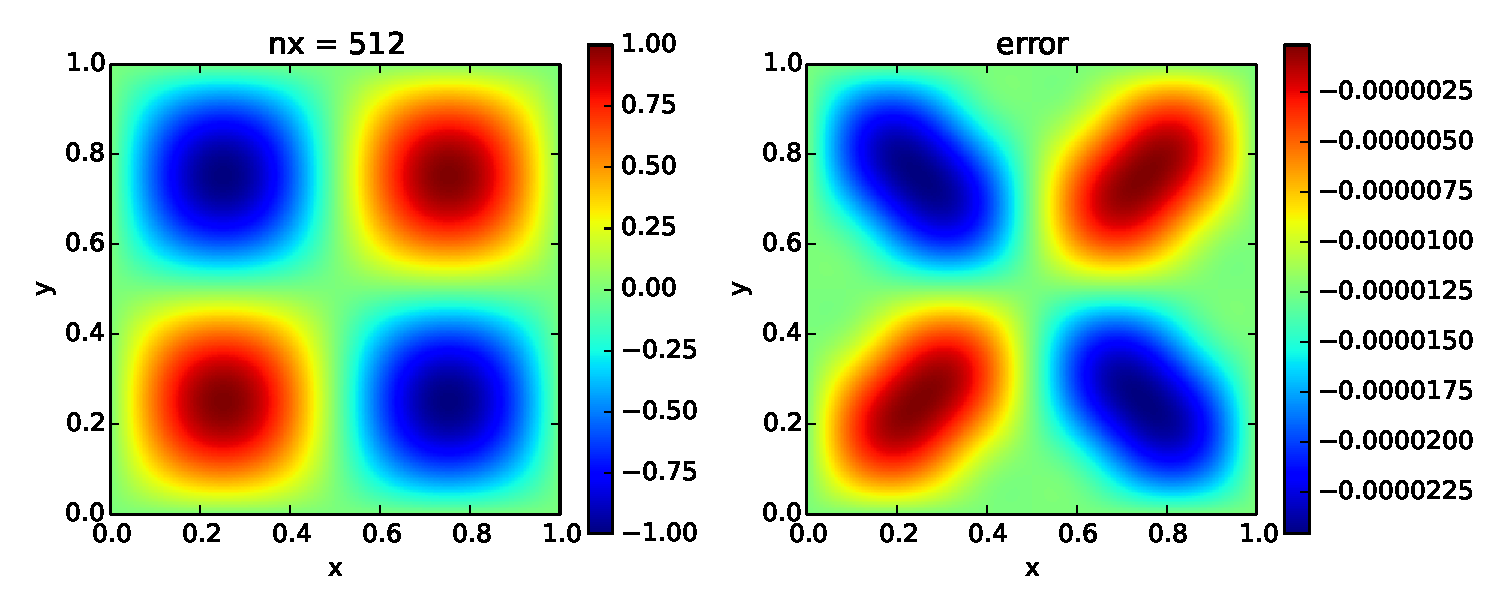
\includegraphics[width=\linewidth]{mg_vc_periodic_test}
\caption[Solution and error of a variable-coefficient Poisson problem]{\label{fig:mg_vc} Solution and error to the variable-coefficient 
Poisson problem defined in Eq.~\ref{eq:vc:lap}.  This test can be
run with \pyro\ {\tt multigrid/mg\_vc\_periodic\_test.py}.}
\end{figure}

\begin{figure}[t]
\centering
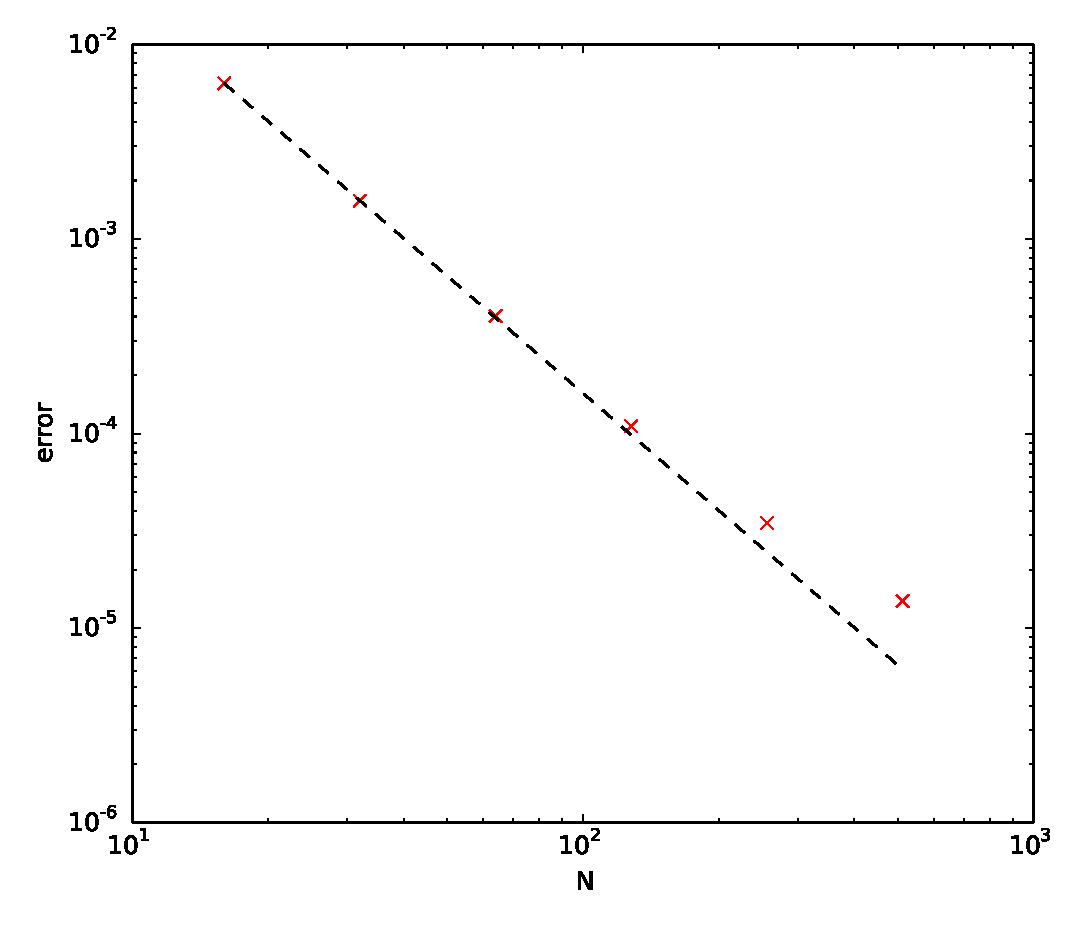
\includegraphics[width=0.8\linewidth]{mg_vc_converge}
\caption[Convergence of the variable-coefficient Poisson solver]{\label{fig:mg_vc_converge} Convergence of the variable-coefficient
multigrid solver for the test problem defined in Eq.~\ref{eq:vc:lap}.  This test can be
run with \pyro\ {\tt multigrid/mg\_vc\_periodic\_test.py}.}
\end{figure}

\subsubsection{Dirichlet}

We can run the same problem with Dirichlet boundary conditions on $\phi$,
and we are free to pick different boundary conditions for $\eta$, since
it represents a different physical quantity.  Since we only have homogeneous
Dirichlet or Neumann BCs implemented, we'll run with Neumann BCs on $\eta$.

\section{Combustion}


Taking $p = p_0 + \pi$, with $p_0 = \mathrm{constant}$, the system 
becomes:
\begin{align}
\frac{\partial \rho}{\partial t} + \nabla \cdot (\rho U) &= 0 \\
\frac{\partial \rho U}{\partial t} + \nabla \cdot (\rho U U) + \nabla \pi &= 0 \\
\nabla \cdot U &= S
\end{align}

\subsection{Species}


\subsection{Constraint}

Our constraint equation is $\nabla \cdot U = S$.  Decomposing the
velocity field as
\begin{equation}
U^\star = U^d + \frac{1}{\rho} \nabla \phi
\end{equation}
our Poisson equation can be defined by taking the divergence, and
using $\nabla \cdot U^d = S$, giving
\begin{equation}
\nabla \cdot \frac{1}{\rho} \nabla \phi = \nabla \cdot U^\star - S
\end{equation}


\subsection{Solution Procedure}

The general solution procedure is for a single step is:
\begin{itemize}

  \item React for $\Delta t/2$

  \item Do the hydrodynamcis for $\Delta t$

    \begin{itemize}
    \item Predict $U$ to the interfaces 
    \item Enforce the divergence constraint on the interface $U$'s (the
      MAC projection) to get $U^\mathrm{adv}$.
    \item Predict $\rho$ to the interfaces
    \item Do the conservative update of $\rho$
    \item Update $U^n$ to $U^{n+1}$
    \item Enforce the divergence constraint on $U^{n+1}$
    \end{itemize}

  \item React for $\Delta t/2$

\end{itemize}

\section{Atmospheric flows}

\subsection{Base State}

For atmospheric flows, we define a one-dimensional base state that is
in hydrostatic equilibrium.  In general, this base state can be
time-dependent, expanding in response to heating in the atmosphere
(see e.g. \cite{almgren:2000,ABRZ:II}.  Here we'll consider only a
time-independent state.

We'll follow the procedure defined in \cite{multilevel}: we define
$\rho_0$ as the lateral average of $\rho$:
\begin{equation}
{\rho_0}_j = \frac{1}{N_x} \sum_i \rho_{i,j}
\end{equation}
and then we define the base state pressure, $p_0$, by integrating the
equation of hydrostatic equilibrium, $dp_0/dy = \rho g$, as:
\begin{equation}
{p_0}_{j+1} = {p_0}_j + \frac{\Delta y}{2} ({\rho_0}_j + {\rho_0}_{j+1}) g
\end{equation}
with an initial condition of 
\begin{equation}
{p_0}_\mathrm{jlo} = \frac{1}{N_x} \sum_{i} p^\mathrm{initial}_{i,\mathrm{jlo}}
\end{equation}



\subsection{Equation Set}

The compressible momentum equation (written in terms of velocity is):
\begin{equation}
\rho \frac{\partial U}{\partial t} + \rho U \cdot \nabla U + \nabla p = \rho g
\end{equation}
Subtracting off the base state, and defining the perturbational
pressure (sometimes called the dynamic pressure) as $p^\prime = p -
p_0$, and perturbational density as $\rho' = \rho - \rho_0$, we have:
\begin{equation}
\rho \frac{\partial U}{\partial t} + \rho U \cdot \nabla U + \nabla p' = \rho' g
\end{equation}
or 
\begin{equation}
\frac{\partial U}{\partial t} + U \cdot \nabla U + \frac{1}{\rho} \nabla p^\prime = 
   \frac{\rho^\prime}{\rho} g
\end{equation}

Several authors \cite{KP:2012,VLBWZ:2013} explored the idea of energy
conservation in a low Mach number system and found that an additional term (which can
look like a buoyancy) is needed in the low Mach number formulation, yielding:
\begin{equation}
\frac{\partial U}{\partial t} + U \cdot \nabla U + 
   \frac{\beta_0}{\rho} \nabla \left (\frac{p^\prime}{\beta_0} \right ) = 
   \frac{\rho^\prime}{\rho} g
\end{equation}

Completing the system are the continuity equation,
\begin{equation}
\frac{\partial \rho}{\partial t} + \nabla \cdot (\rho U) = 0
\end{equation}
and the constraint,
\begin{equation}
\nabla \cdot (\beta_0 U) = 0
\end{equation}
with $\beta_0 = p_0^{1/\gamma}$.

\subsection{Enforcing the Constraint}

Our constraint equation is $\nabla \cdot (\beta_0 U) = 0$.
Decomposing the velocity field as
\begin{equation}
U^\star = U^d + \frac{\beta_0}{\rho} \nabla \phi
\end{equation}
our Poisson equation can be defined by multiplying by $\beta_0$ and
taking the divergence, and using $\nabla \cdot (\beta_0 U^d) = 0$, giving
\begin{equation}
\nabla \cdot \frac{\beta_0^2}{\rho} \nabla \phi = \nabla \cdot (\beta_0 U^\star)
\end{equation}


\subsection{Solution Procedure}

The general solution procedure is for a single step is:
\begin{itemize}

\item Predict $U$ to the interfaces 
\item Enforce the divergence constraint on the interface $U$'s (the
  MAC projection) to get $U^\mathrm{adv}$.
\item Predict $\rho$ to the interfaces
\item Do the conservative update of $\rho$
\item Update $U^n$ to $U^{n+1}$
\item Enforce the divergence constraint on $U^{n+1}$

\end{itemize}
